\chapter{Разработка системы динамической симуляции огня}

Фокус данного исследования направлен на создание реалистично выглядящего огня,
отрисовка которого происходит в режиме реального времени. Это включает в себя
создание компьютерной программы, которая служит для изучения и моделирования
внешнего вида и поведения огня, и при этом плавно работает в режиме реального
времени. В предложенной реализации моделируется поведение костра. Для
моделирования огня была выбрана система частиц, предложенная
в~\cite{reewes1983}.

Моделирование огня в режиме реального времени можно условно разделить на научное
и эстетическое. Несмотря на то, что обе модели стремятся создать реалистичное
пламя, цель и практическое приложение данных моделей отличается. Научные модели
нацелены на исследование динамики определенного феномена. Эти модели нацелены на
точное преставление огня с учетом лежащей в основе поведения огня физики,
включая термодинамику. Целью научных моделей является получение более глубоких
знаний о поведении огня. Научные модели часто используются в экспериментах,
изучении экологических проблем и проблем окружающей среды, военных симуляторах.

Напротив, эстетические модели более сосредоточены на
визуальном\break{}представлении огня, то есть на внешнем виде пламени на экране.
Целью эстетических моделей является воссоздание визуальных эффектов, присущих
огню, используя при этом сравнительно менее ресурсозатратные техники и методики
расчетов по сравнении с научными моделями. Таким образом, эстетические модели
лучше подходят для использования на компьютерах с ограниченными вычислительными
ресурсами а также для использования в приложениях реального времени, которые
крайне чувствительны к задержкам и падению производительности. Примером таких
приложений могут служить видеоигры.

Модель огня костра, разработанную в ходе данного исследования, можно отнести к
эстетической. Основное внимание при разработке системы уделялось воссозданию
поведения и внешнего вида огня, близких к их аналогам в реальном мире. При
создании симуляции использовались некоторые ухищрения, упрощения и ограничения,
которые имеют мало общего с физическими процессами, протекающими в реальном
огне.

\section{Моделирование огня}

При моделировании динамического поведения огня с помощью системы частиц
визуальное восприятие сцены сильно зависит от четырех важных атрибутов частиц:
формы, светимости, прозрачности и цвета. Общая форма огня зависит от размера
частиц и их анимации. Такие эффекты, как мерцание и разделение пламени, зависят
от динамического поведения частиц. Светимость частиц используется для симуляции
эффекта накаливания в пламени. Накаливание --- это эффект нагретыми телами
света. Пламя представляет собой газовый феномен, который имеет высокую
температуру и выделяющий большое количество энергии в окружающую среду. Таким
образом, сквозь пламя могут просвечиваться объекты, находящиеся по другую
сторону огня. Степень прозрачности частиц позволяет моделировать эффект
полупрозрачности, наблюдаемый в реальном пламени.

В данной работе для воссоздания цвета и внешнего вида огня были использованы
текстуры. Наблюдения показывают, что цвет пламени зависит от типа топлива и вида
окислителя, которые взаимодействуют в процессе горения. Углеродное топливо в
основном порождает языки пламени желтого либо оранжевого цветов, в то время, как
различные газы порождают языки пламени голубоватого оттенка. Для упрощения
задачи в рамках исследования производилось моделирование только углеродного
топлива. Далее будет приведено описание разработанной модели на основе системы
частиц.

Разработанная система имеет три ключевых элемента: частицы, эмиттеры, менеджеры
эмиттеров. Данная структура основана на схеме, предложенной
в~\cite{Somasekaran2005UsingPS}. Частицы представлены как небольшие объекты без
четко определенного размера, структуры и траектории движения. Данная
недерминистичная природа частиц была достигнута путем использования
стохастических процессов для вычисления значения атрибутов эмиттера и частиц.
Данное решение позволило достаточно убедительно смоделировать хаотическую
природу огня.

Частицы создаются эмиттерами и затем вводятся в систему частиц.\break{}Эмиттеры
являются случайными точками, расположенными в рамках указанных границ. По факту,
можно считать эмиттеры статическими частицами.\break{}Эмиттеры обладают
различными характеристиками, которые вносят вклад в динамику частиц и общий
внешний вид модели огня. Ключевыми атрибутами эмиттеров являются их позиция,
скорость эмиссии частиц, начальный вектор эмиссии, динамический список частиц, и
энергия эмиттера.

Местоположение эмиттеров, определяет, где в пределах системы частиц будут
создаваться эмиттеры. В предложенной реализации эмиттеры создаются внутри круга,
который обозначает радиус огня. Эмиттеры также управляют скоростью эмиссии
частиц и преобладающим направлением эмиссии. Скорость эмиссии или скорость
горения определяет число частиц, которые испускает каждый эмиттер в момент
времени. Как видно на рисунке~\ref{fig:partLayers}. %TODO:
\begin{figure}[htb]
	\centering
	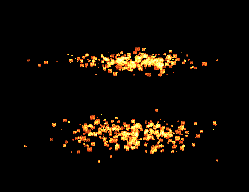
\includegraphics[width=0.4\textwidth]{partLayers}
    \caption{На картинке представлен эффект появления слоев, состоящих из частиц
    испущенных в один момент времени}%
    \label{fig:partLayers}
\end{figure}
